\documentclass[../../../Bachelorarbeit.tex]{subfiles}
\begin{document}

\subsection{Funktionale Sicherheit} \label{sicherheit}
% \color{red}
% An sich nicht Teil des Bachelors. Muss also theoretisch nicht modelliert werden -> Absprache mit Herr Schäfer. Vielleicht trotzdem kurze Aufbereitung der Thematik, wenn Zeit !
Dieses Unterkapitel behandelt die funktionale Sicherheit des mehrachsigen Positioniersystems. Es wird eine Risikobeurteilung vorgenommen, die zu einer Handlungsempfehlung bei der fehlersicheren Inbetriebnahme des Systems führt. Der folgende Inhalt ist lediglich eine Zusammenfassung, die als Überblick dient. Die Mittel zur Minderung \bzw Vermeidung von Risiken gelten als vorgegeben. Ziel dieses Kapitels ist es nicht eine Risikoanalyse mit anschließender Modellierung von Sicherheitsmaßnahmen vorzunehmen.\\
\bigskip \newline
Grundsätzlich können zwei Gefahrenstellen am System erkannt werden. Dies ist zum Einen die Gefährdung von Personen durch einen elektrischen Schock und zum anderen die Gefahr der Verletzung durch die Bewegungen des Systems.\\
Für die Verminderung \bzw Vermeidung von Risiken muss ein Sicherheitskonzept erstellt werden und die aufgestellten Ergebnisse bei der Implementierung mit eingearbeitet werden. Dass heißt konkret, dass die Implementationsphase nicht nur die Hardware-Implementation der eigentlichen Systemkomponenten umfasst, sondern dass sicherheitsbezogene Komponenten mit verbaut/montiert werden. Auch die Software-Implementation wird erweitert um Funktionen die Sicherheit der Anlage betreffend. Das heißt konkret, dass ein Sicherheitsprogramm umgesetzt werden muss.\\
Um Handlungen zur Vermeidung von Risiken durchzuführen, bedarf es zunächst der Ermittlung von Risikoquellen. Wie bereits erwähnt sind das die Verletzungsgefahr durch elektrische Komponenten sowie die Gefahr durch die Bewegung der Achsen der Positioniereinheit geschädigt zu werden. Vor allem die Schädigung durch bewegende Bauteile sorgt für ein erhebliches Risiko, welches es gilt zu minimieren. Dazu wird zunächst ein Risikograph erstellt, um sich der Gefährdung durch das System bewusst zu werden.\\
\bigskip \newline
\textbf{S Schwere der Verletzung}\\
S1 leichte (üblicherweise reversible Verletzung)\\
S2 ernste (üblicherweise irreversible Verletzung oder Tod)\\
\textbf{F Häufigkeit und/oder Dauer der Gefährdungsexposition}\\
F1 selten bis weniger häufig und/oder die Zeit der Gefährdungsexposition ist kurz\\
F2 häufig bis dauernd und/oder die Zeit der Gefährdungsexposition ist lang\\
\textbf{P Möglichkeit zur Vermeidung der Gefährdung oder Begrenzung des Schadens}\\
P1 möglich unter bestimmten Bedingungen\\
P2 kaum möglich

\begin{figure}[H]
    \centering
    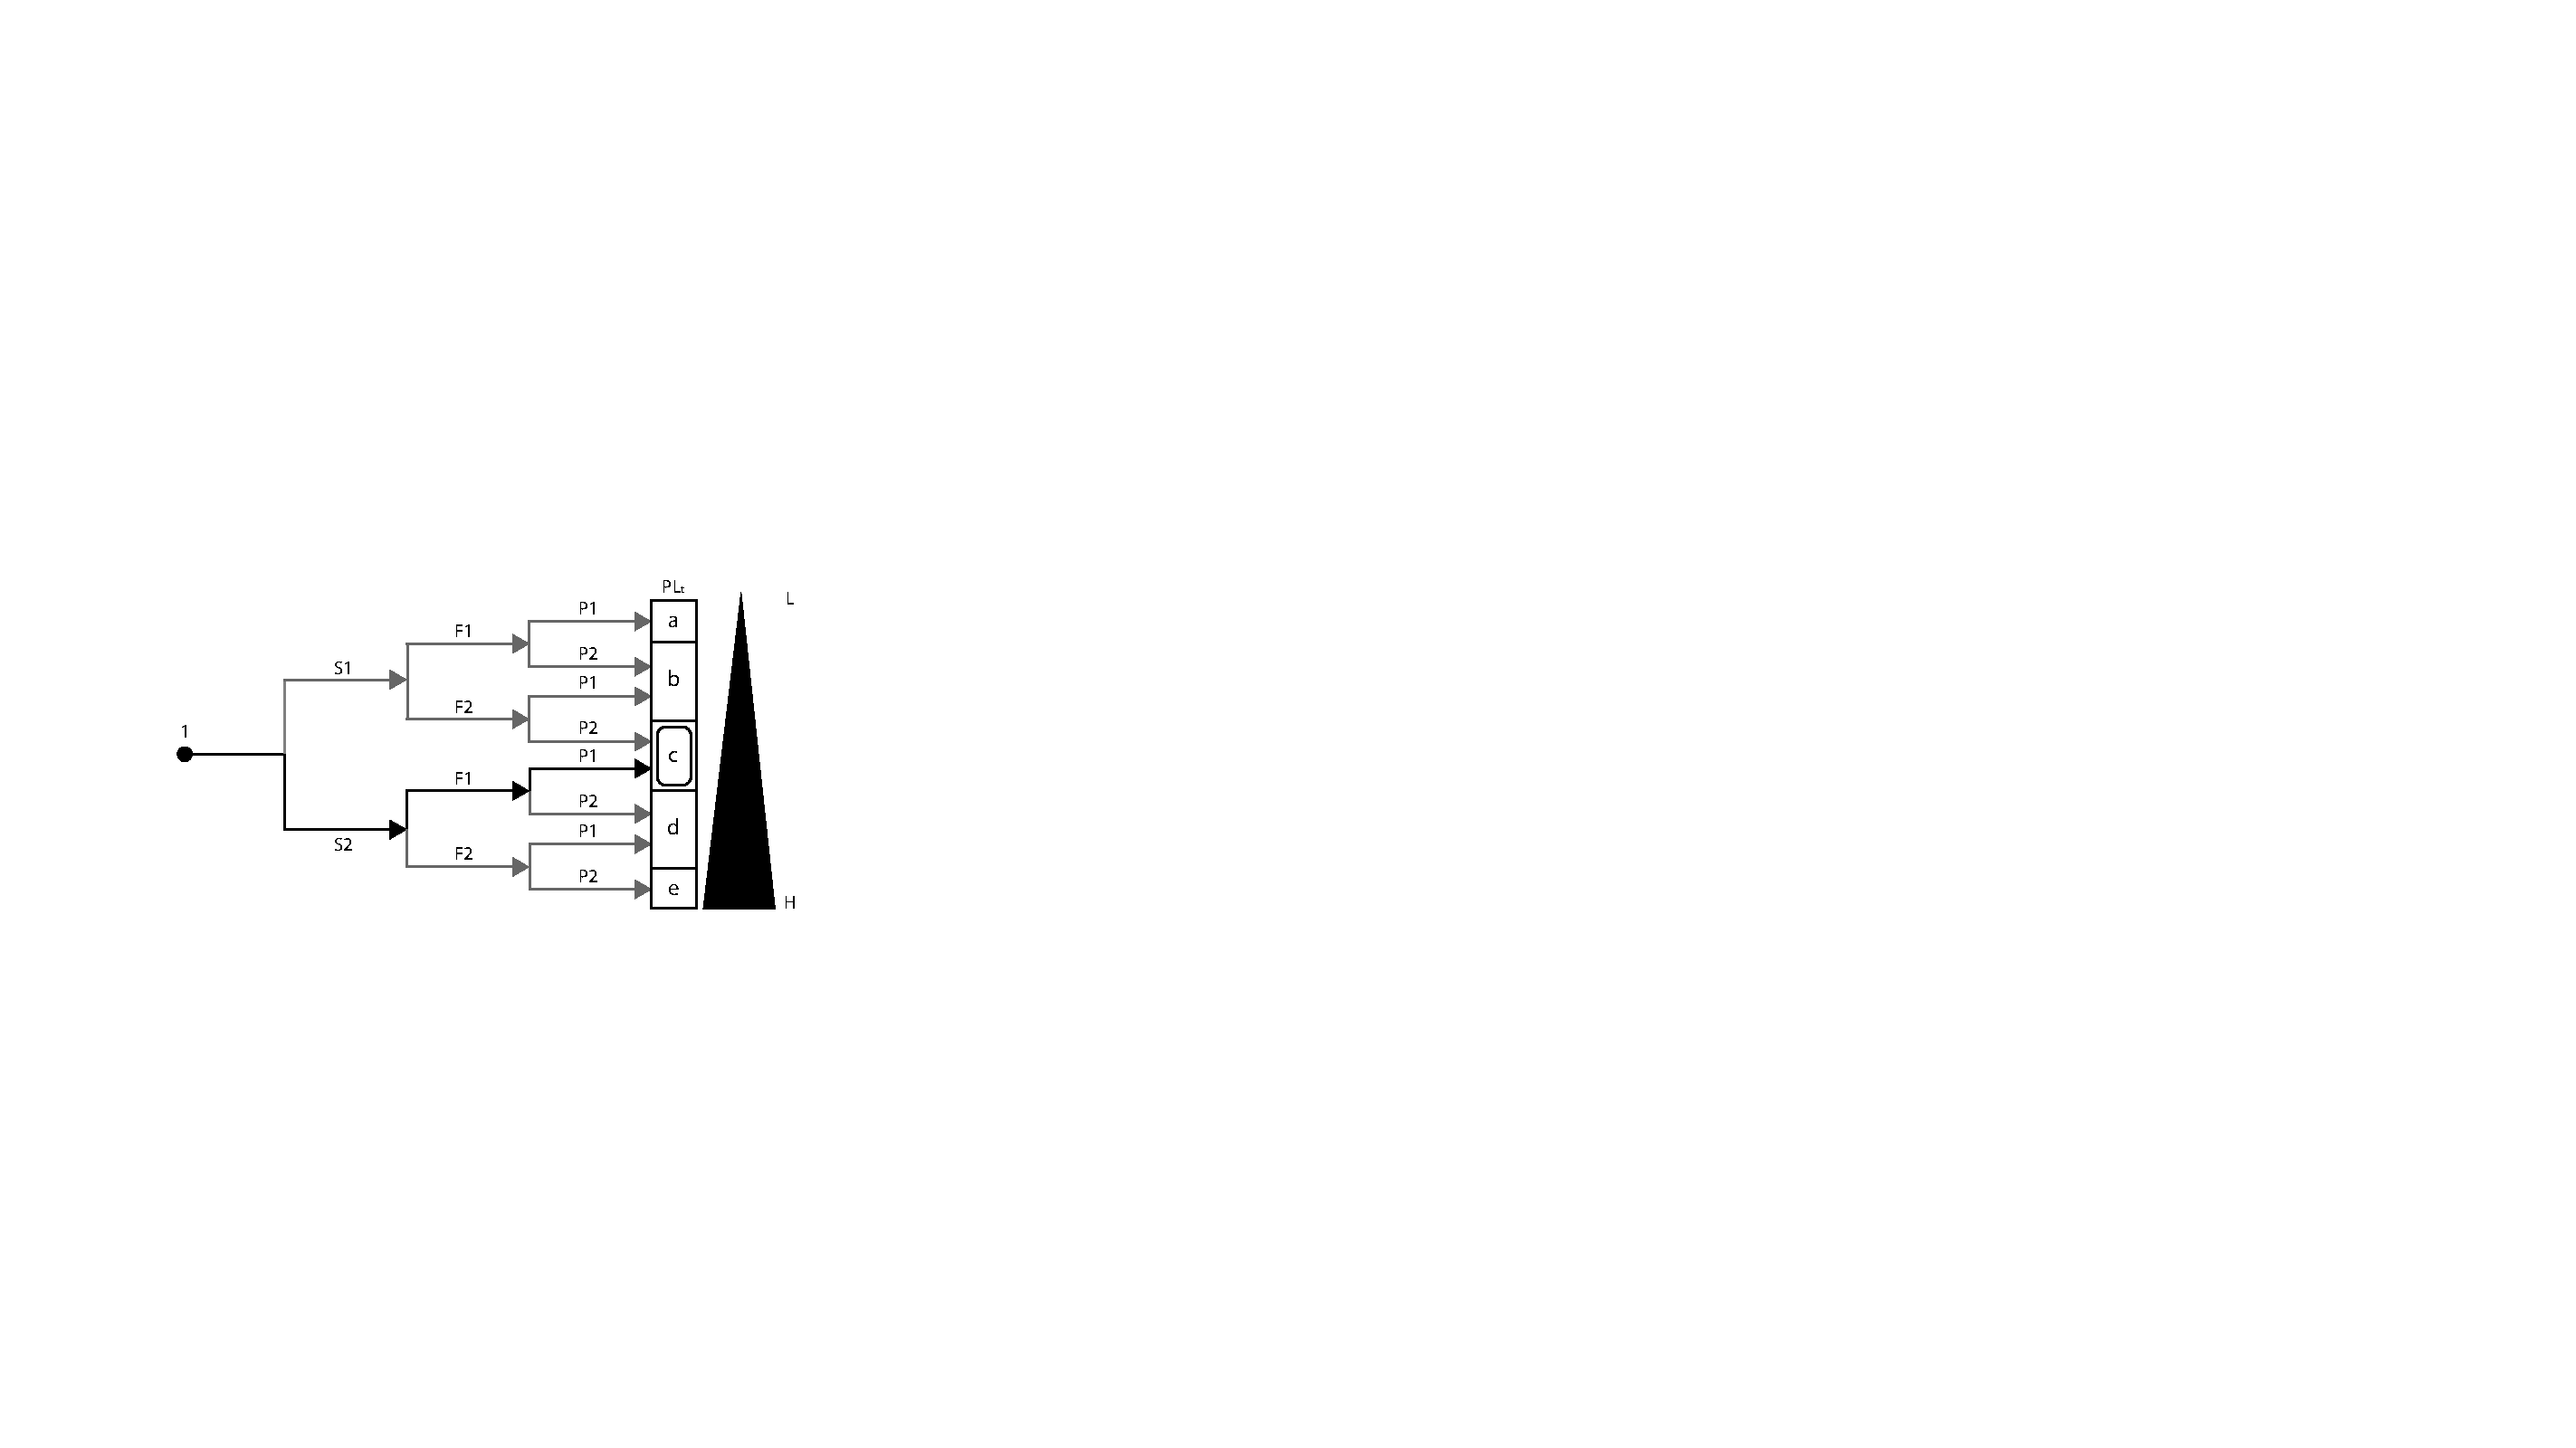
\includegraphics[width=0.7\textwidth]{Images/Risikograph.pdf}
    \caption[Risikograph]{Risikograph nach DIN EN ISO 13849-1 zum mehrachsigen Positioniersystem}
    \label{fig:my-img103}
\end{figure}

Es ist zu erkennen, dass von der Laboranlage ein mittelschweres Risiko ausgeht für insbesondere Personen in direktem Kontakt mit dem System. Zur Verminderung von Gefahren durch sich bewegende Elemente können mehrere Strategien angewendet werden. Dennoch gibt es eine Systemkomponente, die für ein System dieser Art immer Anwendung finden muss. Es handelt sich um einen Not-Halt. Im Unterschied zu einem Not-Stop ist es wichtig festzustellen, dass die Gefahrensituation von beweglichen Elementen ausgeht und nicht von Strömen und Spannungen. Es wäre sogar fatal das System spannungsfrei zu schalten, da dies mögliche unkontrollierte Bewegungen und somit undefinierte Zustände als Folge hätte. Somit ist es Priorität sämtliche Bewegungen in einer Notsituation zu stoppen.\\
Da die reine Not-Halt Funktionalität ausgelöst durch ein Tast-Ereignis nicht ausreichend ist, um das System sicher für den Nutzer zu machen, ist eine weitere Handlung nötig. Vorgabe für das mehrachsige Positioniersystem ist laut Anforderungen die Nutzung eines Lichtvorhanges. Dieser soll das Eintreten in den Arbeitsbereich des Systems erkennen und den Not-Halt auslösen. Eine weitere Maßnahme ist die Verwendung einer dedizierten Sicherheitssteuerung (konkret: \acs{SLC}100). Diese ermöglicht eine redundante Berechnung von fehlerrelevanten Funktionen. Durch die Redundanz können kritische Systemfehler minimiert werden.\\
Zur effektiven Minderung der Risiken werden nun folgende Reaktionszeiten an das System vorgegeben:\\
\bigskip \newline
Maximale Auslösezeit des Lichtvorhangs: 50 \si{ms}\\
Maximale Bremsdauer bei Not-Halt: 200 \si{ms}\\
Maximale Abschaltzeit des Servoreglers bei Not-Halt: 250 \si{ms}\\

Das System sei nach Vorgaben nun maximal sicher nach der Implementierung der aufgezählten Maßnahmen. Das bedeutet jedoch nicht, dass es zu 100\% sicher ist. Die Umsetzung der funktionalen Sicherheit ist in \autoref{implementation} dokumentiert.

% TODO: Hier muss noch mehr hin !!!

\end{document}